\chapter*{Solutions to Set \#12}
\addcontentsline{toc}{chapter}{Solutions to Set \#12}
\markboth{Solutions to Set \#12}{Solutions to Set \#12}
\label{set11sols}



\begin{sol}{ex:binom2}\index{Strassmann series!representing $(1+a)^n$} We begin with a simple lemma.

\begin{lem} If $x \in 1+p^k \Z_p$, where $k \in \Z^{+}$, then $x^p \in 1+p^{k+1}\Z_p$.\end{lem}
\begin{proof} Write $x=1+p^k r$, where $r \in \Z_p$. Then $x^p = 1 + p^{k+1}r + \sum_{j \ge 2} \binom{p}{j} p^{jk} r^j \equiv 1 \pmod{p^{k+1}\Z_p}$, as desired.\end{proof}

Now we return to the problem at hand. Since $a\in p\Z_p$, applying the lemma $m$ times will show  $(1+a)^{p^m} \in 1 + p^{m+1}\Z_p$. Hence, $|(1+a)^{p^m}-1|_p \le p^{-m-1}$, so that $(1+a)^{p^m}\to 1$. Therefore, for any $n \in \Z$,
\[ (1+a)^{n} = (1+a)^{n} \lim_{m\to\infty} (1+a)^{p^m} = \lim_{m\to\infty} (1+a)^{n+p^m}. \]
This proves the first equality claimed in the problem.

Whenever $n+p^m\ge 0$, we have $(1+a)^{n+p^m} = \Binom(1+a;n+p^m)$, by Exercise \ref{ex:binomialseries}. This explains the second equality.

Write $\Binom(1+a;n +p^m)-\Binom(1+a;n) =\sum_{j\ge 0} C_{a,j} ((n+p^m)^j-n^j)$. Then
\begin{align*} |\Binom(1+a;n +p^m)-\Binom(1+a;n)|_p &\le \max_{j\ge 0} |C_{a,j}|_p |(n+p^m)^j-n^j|_p \\& \le p^{-m} \max_{j\ge 0} |C_{a,j}|_p, \end{align*}
which tends to $0$ as $m\to\infty$. This yields the final equality.
\end{sol}

\begin{challenge} Let $p$ be an odd prime, and let $a \in p\Z_p$. You have just demonstrated one way to extend $(1+a)^x$ from a function of $x$ defined on $\Z$ to one defined on $\Z_p$: Set $(1+a)^x := \Binom(1+a;x)$. But there is another approach you could take to extend the domain of $(1+a)^x$ to $\Z_p$. Namely, you might define $(1+a)^x$ as the limit of $(1+a)^{x_n}$, where $x_n$ is any sequence of integers converging to $x$ in $\Q_p$. This should remind you of how exponentiation of real numbers is defined when the exponent is irrational.

Check that this idea works (i.e., leads to a well-defined value of $(1+a)^x$, independent of the particular sequence $x_n$) but doesn't give anything new: $(1+a)^x = \Binom(1+a;x)$, again. What happens when $p=2$?
\end{challenge}

\begin{sol}{ex:KC} Put $F(T) = \sum_{i=1}^{m} a_i \cdot \Binom(\beta_i;T)-A$. The results of Problems \ref{ex:binomialseries} and \ref{ex:binom2} imply that $F(T)$ is a Strassmann series with $F(n) = \sum_{i=1}^{m} a_i \beta_i^n - A$ for every $n \in \Z$. 

Every $n\in \Z$ satisfying $a_1\beta_1^n + \dots + a_m \beta_m^n = A$ is a zero of $F$ in $\Z_p$. So if this equation has infinitely many integer solutions, then $F$ has infinitely many zeros in $\Z_p$. In that case, $F(T) = 0$ in $\Q_p[[T]]$ (by Exercise \ref{ex:weakstrass}). Then $A=  F(n) + A = a_1\beta_1^n + \dots + a_m \beta_m^n$ for all $n \in \Z$.
\end{sol}

\begin{rmk} It is often easy to rule out that $\sum_{i=1}^{m} a_i \beta_i^n = A$ for all $n \in \Z$. Let's assume, as is natural to do, that no $a_i=0$. 

Suppose to start off that $A=0$. If $\sum_{i=1}^{m} a_i \beta_i^n = 0$ for all $n\in \Z$ (or even just the nonnegative $n \in \Z$), then we have a formal identity
\[ 0= \sum_{n\ge 0} \left(\sum_{i=1}^{m} a_i \beta_i^{n}\right) T^n = \sum_{i=1}^{m} a_i \sum_{n\ge 0} (\beta_i T)^n = \sum_{i=1}^{m} \frac{a_i}{1-\beta_i T}. \]
Multiplying through by $\prod_{j=1}^{m} (1-\beta_j T)$ and replacing $T$ with $1/\beta_1$ shows that $0 = a_1 \prod_{j=2}^{m}(1-\beta_j/\beta_1)$. Hence, $\beta_1 = \beta_j$ for some $j=2,3,\dots,m$. That is, the term $\beta_1$ is repeated in the list $\beta_1,\dots,\beta_m$. But our setup is symmetric, and so  \emph{every} $\beta_i$ must appear at least twice in that list. Turning things around, if some $\beta_i$ appears only once, then we cannot have $\sum_{i=1}^{n} a_i \beta_i^n = 0$ for all $n\in \Z$. For an application, see the Remark following the solution of Problem \ref{ex:cubicpell2}.

Similar reasoning can be applied when $A \ne 0$. If $\sum_{i=1}^{m} a_i \beta_i^n = A$ for all nonnegative integers $n$, we find that $\frac{A}{1-T} = \sum_{i=1}^{m} \frac{a_i}{1-\beta_i T}$. This leads to the conclusion that every element in the list $1,\beta_1,\dots,\beta_m$ is repeated.
\end{rmk}

\begin{sol}{prob:coeffsisolate}\index{$\Z[\sqrt[3]{D}]$, arithmetic of} If $\alpha = x+y\theta + z\theta^2$, then $\alpha' = x + y\theta' + z\theta'^2 = x+y\omega\theta + z\omega^2 \theta^2$, and $\alpha'' = x + y\theta'' + z\theta''^2 = x+y\omega^2\theta + z\omega \theta^2$. Hence,
\[ \alpha+\alpha' + \alpha'' = 3x + y\theta(1+\omega+\omega^2) + z\theta^2(1+\omega^2+\omega)= 3x.\]
Similarly,
\begin{align*} \alpha + \omega^2 \alpha' + \omega \alpha'' &= (x+y\theta + z\theta^2) + (x \omega^2 + y\theta + z\omega \theta^2) + (x\omega + y\theta + z\omega^2 \theta^2) \\
&= x(1+\omega^2+\omega) + 3y\theta + z\theta^2 (1+\omega + \omega^2) \\&=3y\theta,
\end{align*}
and
\begin{align*}
\alpha + \omega\alpha' + \omega^2\alpha'' &= (x+y\theta+z\theta^2) + (x\omega + y\omega^2\theta + z\theta^2) + (x\omega^2 + y\omega \theta + z\theta^2) \\
&= x(1+\omega+\omega^2) + y\theta(1+\omega^2+\omega) + 3z\theta^2 \\
&= 3z\theta^2.
\end{align*}
\end{sol}

\begin{sol}{prob:discretelattice} Suppose $|\alpha|, |\alpha'|\le R$. Since $\alpha''$ is the complex conjugate of $\alpha'$, we also have $|\alpha''|  \le R$. By Exercise \ref{prob:coeffsisolate}, $|x| \le \frac{1}{3} (|\alpha|+|\alpha'|+|\alpha''|) \le R$, $|y| \le \frac{1}{3|\theta|}(|\alpha| +|\omega^2\alpha'| + |\omega\alpha''|) \le \frac{R}{|\theta|}$, and $|z| \le \frac{1}{3|\theta|^2}(|\alpha| + |\omega\alpha'| + |\omega^2\alpha''|) \le \frac{R}{|\theta|^2}$. So there are finitely many possibilities for the integers $x, y$, and $z$, and therefore  finitely many possibilities for $\alpha = x + y\theta + z\theta^2$.
\end{sol}

\begin{sol}{prob:dirichletidea} For all $\varepsilon_1,\varepsilon_2 \in \Uu$, 
\begin{align*} \Ll(\varepsilon_1 \varepsilon_2) &= (\log \varepsilon_1\varepsilon_2, 2\log|(\varepsilon_1 \varepsilon_2)'|) \\&= (\log \varepsilon_1,2\log|\varepsilon_1'|) + (\log \varepsilon_2,2\log|\varepsilon_2'|) = \Ll(\varepsilon_1) + \Ll(\varepsilon_2).\end{align*} So $\Ll$ is a homomorphism. If $\Ll(\varepsilon) = 0$, then $\log{\varepsilon}=0$, which implies $\varepsilon=1$. Therefore, $\ker(\Ll)$ is trivial and $\Ll$ is injective. Finally, summing the $x$ and $y$ coordinates of $\Ll(\varepsilon)$ gives $\log \varepsilon + 2 \log|\varepsilon'| = \log(\varepsilon|\varepsilon'|^2) = \log \Nm{\varepsilon}= \log 1 = 0$. So the image of $\Ll$ is contained in the subspace $x+y=0$.
\end{sol}


\begin{figure}
\centering
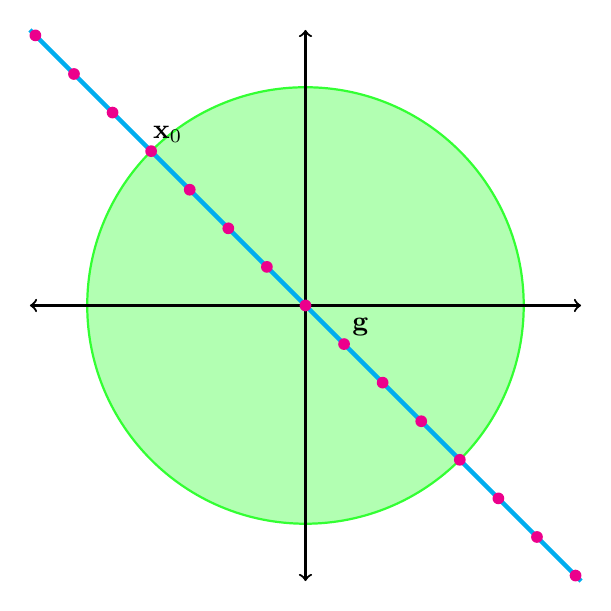
\begin{tikzpicture}[scale=0.7]
\draw[green!80,thick,fill=green!30] (0,0) circle (3.9597);

\draw[color=cyan, ultra thick] (-5,5) -- (5,-5);
\draw[color=black, thick,->] (0,0) -- (5,0);
\draw[color=black, thick,->] (0,0) -- (-5,0);
\draw[color=black, thick,->] (0,0) -- (0,5);
\draw[color=black, thick,->] (0,0) -- (0,-5);
\node at (0,0) [color=magenta,circle,fill,inner sep=1.5pt]{};

\node at (-0.7,0.7) [color=magenta,circle,fill,inner sep=1.5pt]{};
\node at (-1.4,1.4) [color=magenta,circle,fill,inner sep=1.5pt]{};
\node at (-2.1,2.1) [color=magenta,circle,fill,inner sep=1.5pt]{};
\node at (-2.8,2.8) [color=magenta,circle,fill,inner sep=1.5pt]{};
\node at (-3.5,3.5) [color=magenta,circle,fill,inner sep=1.5pt]{};
\node at (-4.2,4.2) [color=magenta,circle,fill,inner sep=1.5pt]{};
\node at (-4.9,4.9) [color=magenta,circle,fill,inner sep=1.5pt]{};
\node at (0.7,-0.7) [color=magenta,circle,fill,inner sep=1.5pt]{};
\node at (1.4,-1.4) [color=magenta,circle,fill,inner sep=1.5pt]{};
\node at (2.1,-2.1) [color=magenta,circle,fill,inner sep=1.5pt]{};
\node at (2.8,-2.8) [color=magenta,circle,fill,inner sep=1.5pt]{};
\node at (3.5,-3.5) [color=magenta,circle,fill,inner sep=1.5pt]{};
\node at (4.2,-4.2) [color=magenta,circle,fill,inner sep=1.5pt]{};
\node at (4.9,-4.9) [color=magenta,circle,fill,inner sep=1.5pt]{};
\node at (-2.5,3.1) [color=black]{$\mathbf{x}_0$};
\node at (1.0,-0.4) [color=black]{$\mathbf{g}$};
\node at (2,2) [color=black]{$\Dd$};
\end{tikzpicture}
\caption*{Figure corresponding to the solution of Problem \ref{prob:grouplemma}.}
\end{figure}


\begin{sol}{prob:grouplemma} We show that if (i) and (iii) both fail, then (ii) must hold. Since (i) fails, we may choose an $\mathbf{x}_0 \in \mathcal{G}$ with $\mathbf{x}_0 \ne \mathbf{0}$. Let $\Dd$ denote the closed disc about $\mathbf{0}$ passing through $\mathbf{x}_0$. The set $(\mathcal{G}\setminus\{\mathbf{0}\}) \cap \Dd$ is nonempty (containing, for example, $\mathbf{x}_0$). Since (iii) fails, this set is also finite. Let $\mathbf{g}$ be any element of $(\mathcal{G}\setminus\{\mathbf{0}\}) \cap \Dd$ minimizing the Euclidean distance to $\mathbf{0}$ (among elements of $(\mathcal{G}\setminus\{\mathbf{0}\}) \cap \Dd$). 

As $\mathbf{g}$ is a nonzero vector belonging to the one-dimensional subspace $V:= \{(x,y): x+y=0\}$ of $\R^2$, we have that $V = \R\mathbf{g}$. We leverage this observation to show that $\mathbf{g}$ generates $\mathcal{G}$. (Hence, (ii) holds!) It is enough to show that an arbitrarily chosen $\mathbf{x} \in \mathcal{G}$ belongs to $\langle \mathbf{g}\rangle$. Since $\mathcal{G} \subset V$, we may write $\mathbf{x} = t\mathbf{g}$, where $t \in \R$. Then $\{t\} \mathbf{g} = \mathbf{x} - \lfloor t\rfloor \mathbf{g} \in \mathcal{G}$. (Here $\{t\} = t -\lfloor t\rfloor$ denotes the fractional part of $t$.) Since $0 \le \{t\} < 1$, the vector $\{t\}\mathbf{g}$ is an element of $\mathcal{G}$ closer to the origin than $\mathbf{g}$. This contradicts the choice of $\textbf{g}$ unless $\mathbf{x} -\lfloor t\rfloor\mathbf{g} =\mathbf{0}$. But then $\mathbf{x} = \lfloor t\rfloor \mathbf{g} \in \langle \mathbf{g}\rangle$. 
\end{sol}


\begin{sol}{prob:almostunittheorem} In view of Problem \ref{prob:grouplemma}, it is enough to show that each closed disc about $\mathbf{0}$ intersects $\Ll(\Uu)$ in a finite set.

Let $\Dd$ be the closed disc of radius $R$ centered at $\mathbf{0}$. Every element of $\Dd \cap \Ll(\Uu)$ can be written as $\Ll(\varepsilon)$ where $1 \le \varepsilon \le e^R$ and $|\varepsilon'| \le e^{R/2}$. As a consequence of Problem \ref{prob:discretelattice}, there are only finitely many possibilities for $\varepsilon$ and hence only finitely many possibilities for $\Ll(\varepsilon)$. 
\end{sol}

\begin{sol}{prob:all1} Since $\theta^3=D$ and $D$ is cubefree, $0 \le 3 v_p(\theta) = v_p(D) < 3$. Hence, $v_p(\theta)=0$ and $|\theta|_p=1$. Also, $|\omega|_p^3 = |\omega^3|_p = |1|_p = 1_p$, so that $|\omega|_p=1$.

Each of $\mu, \mu', \mu'' \in \Z[\theta, \omega]$. Since $\Z\subset \Z_p$ and $\theta, \omega \in \Z_p^{\times}$, we have $\Z[\theta,\omega] \subset \Z_p$. Hence, $|\mu|_p, |\mu'|_p, |\mu''|_p \le 1$. But $|\mu|_p |\mu'|_p |\mu''|_p = |\mu \mu' \mu''|_p = |1|_p=1$. So it must be that $|\mu|_p, |\mu'|_p, |\mu''|_p = 1$.
\end{sol}

\begin{sol}{prob:notconstantzero}\index{$x^3-Dy^3=1$, finiteness of solutions}\index{cubic Pellian equation} Fix $r \in \Z$. For each $m\in \Z$, set $E(m) = \mu^r \nu^m + \omega \mu'^r \nu'^m + \omega^2 \mu''^r \nu''^m$. The equation $E(m)=0$ is an equation involving only elements of $L$ and field operations in $L$. At present, our attention is fixed on the embedded copy of $L$ inside $\Q_p$, but if $E(m)=0$ holds in that copy of $L$, it holds in the OG\footnote{Original Gauss} version of $L$, which is a subfield of $\C$.  

Back in the complex numbers, $|\mu| = \mu > 1$. (Here and below $|\cdot|$ is the usual complex absolute value.) Moreover, $1 = \mu|\mu'\mu''| = \mu |\mu'|^2$, so that $|\mu'| = |\mu''| = 1/\mu < 1$. It follows that $|\nu| = \nu >1$ while $|\nu'| = |\nu''| < 1$. As a consequence, 
\[ |\omega \mu'^r \nu'^m + \omega^2 \mu''^r \nu''^m| \le |\mu'^r|\cdot |\nu'|^m + |\mu''^r| \cdot |\nu''|^m < 1\]
for all large enough positive integers $m$, and
\[ |E(m)| \ge |\mu^r \nu^m| - |\omega \mu'^r \nu'^m + \omega^2 \mu''^r \nu''^m| \ge |\mu^r| \nu^m - 1 > 0 \]
for all sufficiently large $m$.

Therefore, if we pick $m$ as a large enough positive integer, then $E(m)\ne 0$ (and this holds whether we are thinking of $L$ as inside $\C$ or inside $\Q_p$). So from the Strassmann series machinery that we have built up, $E(m)=0$ for only finitely many integers $m$. (Note that this finiteness does \emph{not} follow from the bounds over $\C$ that we derived above. Those bounds imply that $E(m)=0$ for only finitely many positive integers $m$, but they say nothing useful about negative integers $m$.) Finally, letting $r$ range from $0$ to $p-1$, we see that $\mu^n + \omega \mu'^n + \omega^2 \mu''^n=0$ for only finitely many $n\in \Z$.
\end{sol}


\begin{rmk} We can shorten the argument using the Remark following the solution to Problem \ref{ex:KC}. If $E(m)=0$ for all $m \in \Z$, then each term in the list $\nu, \nu', \nu''$ is repeated. But, working again in $\C$,
\[ |\nu| = \nu > 1 > |\nu'| = |\nu''|,\] and so $\nu$ is not repeated.
\end{rmk}

\begin{sol}{prob:strikingcor} Suppose $n^3+1$ has all prime factors from $\mathcal{P}$. Then $n^3+1 = \prod_{p \in \Pp} p^{v_p}$ for some nonnegative integers $v_p$. Writing each $v_p = 3e_p +r_p$, where $r_p \in \{0,1,2\}$, 
\[ n^3+1 = (-D)y^3 \qquad\text{for}\qquad D =\prod_{p\in \Pp} p^{r_p}, \quad y = -\prod_{p\in\Pp}p^{e_p}. \] 
Hence, $(-n,y)$ is an integer solution to $X^3-DY^3=1$. 

By construction, $D\in \mathcal{D}$. If $D=1$, then $n^3$ and $n^3+1$ are positive perfect cubes differing by $1$. But the smallest difference between positive perfect cubes is $2^3-1^3=7$. Thus, $D \in \mathcal{D}\setminus \{1\}$.

By Problem \ref{prob:notconstantzero}, each equation $X^3-DY^3=1$, with $D \in \mathcal{D}\setminus \{1\}$, has finitely many integer solutions. Since $\#\mathcal{D}$ is finite, we conclude that there are finitely many $n$ for which $n^3+1$ has all prime factors from $\Pp$. To deduce that the largest prime factor of $n^3+1$ tends to infinity, choose $\Pp$ as the set of primes up to an arbitrarily prescribed bound.
\end{sol}


\begin{challenge}\index{$x^3-Dy^3=k$, finiteness of solutions} Keep the same assumptions and notation from the proof of the theorem. In this exercise, you will show that for each nonzero integer $k$, the equation $x^3-Dy^3=k$ has finitely many integer solutions $x,y$. Equivalently, there are finitely many pairs of integers $x,y$ with $\Nm(x-y\theta)=k$.
\vspace{-0.12in}
\begin{enumerate}
\item[(a)] Show that the ring $\Z[\theta]/k\Z[\theta]$ is finite, and that in fact $\#\Z[\theta]/k\Z[\theta] = |k|_{\infty}^3$.
\item[(b)] Prove that if $\kappa \in \Z[\theta]$ has $\Nm\kappa=k$, then $\kappa \Z[\theta] \supset k\Z[\theta]$. Deduce from (a) that there are finitely many possibilities for $\kappa$, up to associates. 
\item[(c)] Suppose $\kappa \in \Z[\theta]$ has $\Nm\kappa=k$. Prove that there  are finitely many $u \in \mathcal{U}$ (same meaning as above --- positive units in $\Z[\theta]$) for which $u\kappa$ has the form $x-y\theta$ for some $x,y \in \Z$. Conclude!
\end{enumerate}
\end{challenge}

\begin{challenge}[continuation] Fix a finite set of primes $\mathcal{P}$ and a nonzero integer $d$. Show that there are finitely many $n \in \Z$ such that both $n$ and $n+d$ have all of their prime factors belonging to $\mathcal{P}$.
\end{challenge}


\begin{rmk} As stated on Set \#12, Delaunay and Nagell showed that $x^3-Dy^3=1$ has at most one integer solution with $y\ne 0$. It was discovered by Skolem \cite{skolem} that their theorem can be established by $p$-adic methods. Skolem's proof uses arithmetic in extensions of $\Q_3$; a more elementary $p$-adic proof can be found in lecture notes of Ljunggren \cite{ljunggren}.
\end{rmk}



\let\oldaddcontenttsline\addcontentsline
\renewcommand{\addcontentsline}[3]{}
\begin{thebibliography}{11}
\bibitem{ljunggren} W. Ljunggren,
\emph{Diophantine equations: a $p$-adic approach}. Notes by {R.\,R.} Laxton from a 1968 lecture course at the University of Nottingham.

\bibitem{skolem} T. Skolem,
\emph{Anvendelse av 3-adisk analyse og \textsubscript{''}bikropper`` til bevis for noen satser angående visse kubiske ubestemte ligninger}. Norsk Mat. Tidsskr. \textbf{34} (1952), 45--51.

\end{thebibliography}
\let\addcontentsline\oldaddcontentsline